\documentclass{beamer}

\usecolortheme[dark,accent=cyan]{solarized}

\beamertemplatenavigationsymbolsempty

\usepackage{graphicx}
\usepackage{microtype}
\usepackage{multimedia}
\usepackage{pgfplots}
\usepackage{hyperref}
\usepackage{colortbl, xcolor}
\usepackage{booktabs}
\usepackage{varwidth}

\usepackage{animate}
\usepackage{tikz}
\usetikzlibrary{positioning}
\usetikzlibrary{calc}
\usepackage{minted}

\definecolor{DarkGray}{gray}{0.1}
\definecolor{LightGray}{gray}{0.3}
\usemintedstyle{native}

\theoremstyle{definition}
\newtheorem{defn}{Definition}

\title{Writing tests for research software}
\author{@NikoletaGlyn}
\date{}
\institute[]
{
\begin{center}
    
\includegraphics[width=.15\textwidth]{static/pycon-namibia.png}
\end{center}
}

\begin{document}

\frame{\titlepage}

\begin{frame}{}
    \begin{center}
    
\includegraphics[width=0.24\textwidth]{static/cardiff_uni_logo.jpg}\hspace{10pt}
    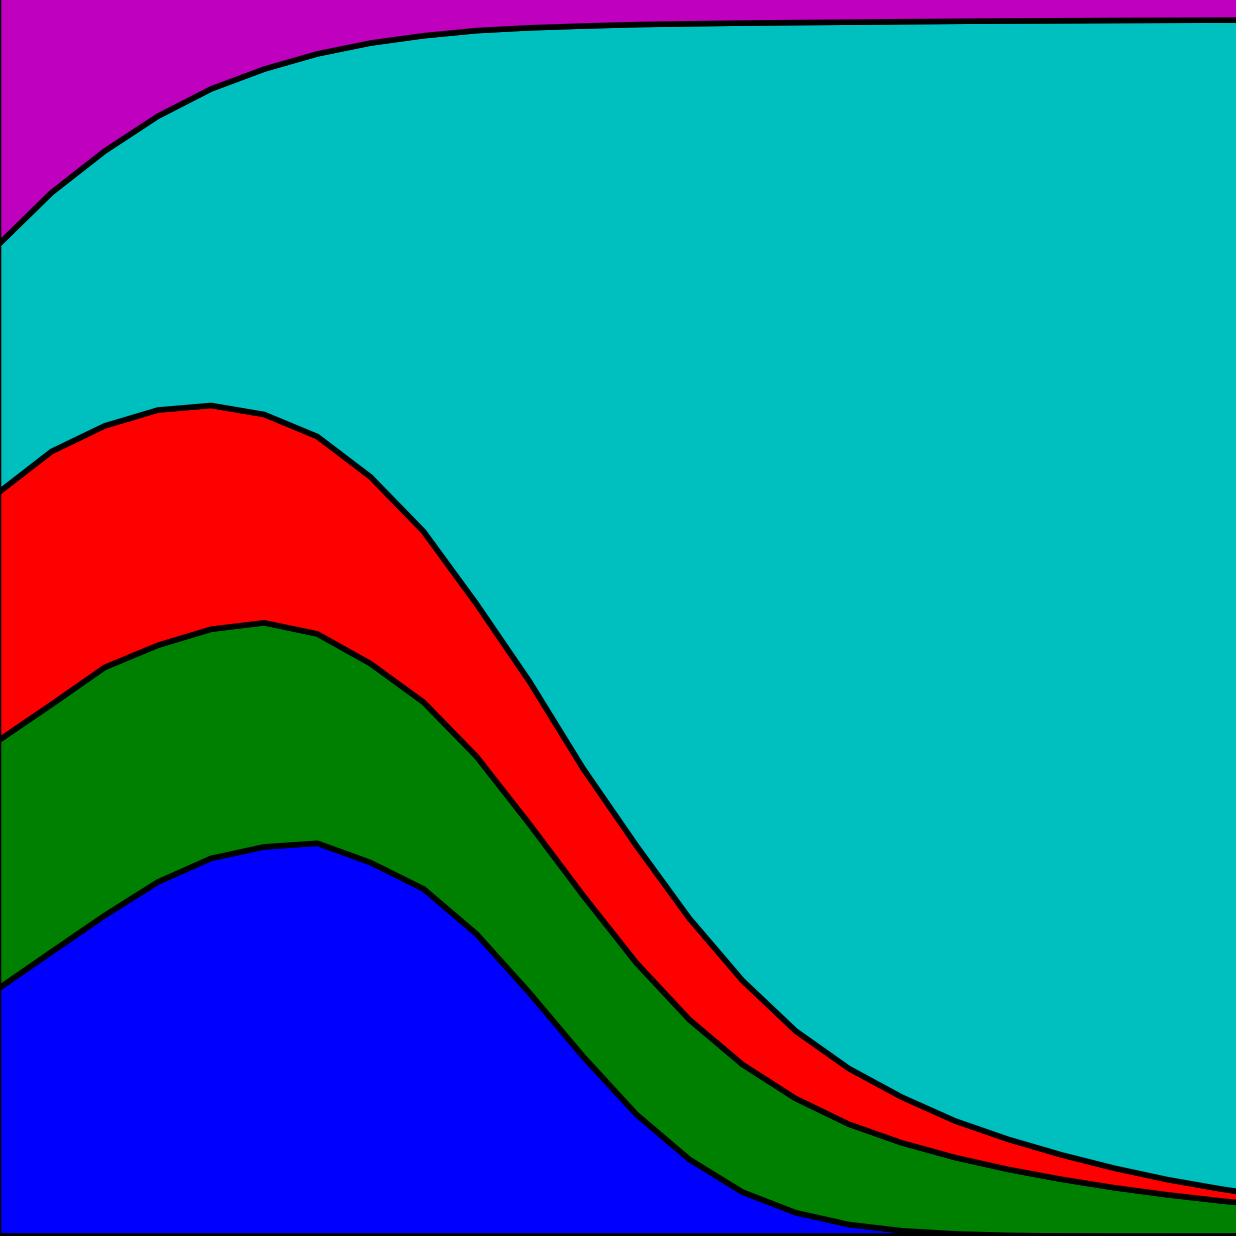
\includegraphics[width=0.24\textwidth]{static/axelrod-logo.png}\vspace{10pt}

    
\includegraphics[width=0.24\textwidth]{static/ssi-logo.png} \hspace{10pt}
    
\includegraphics[width=0.24\textwidth]{static/phoenix-logo.jpg}
    \vspace{10pt}
    \end{center}
\end{frame}

\begin{frame}
    \begin{center}
        \huge {TESTING}
    \end{center}
\end{frame}

\begin{frame}
    \begin{center}
        \color{yellow!79}\huge{0, 1, 1, 2, 3, 5, 8, 13, 21, 34 ...}
    \end{center}
\end{frame}

\begin{frame}
    \begin{center}
        \color{yellow!79}\huge{$F_{n} = F_{n-1} + F_{n-2}$}
    \end{center}
\end{frame}

\begin{frame}[fragile]
    \begin{figure}
    \textbf{'main.py'}
    \begin{minted}
        [
        framesep=2mm,
        baselinestretch=1,
        bgcolor=DarkGray,
        fontsize=\small,
        ]
        {python}
def fib(n):
   if n == 1:
      return 1
   elif n == 0:
      return 0
   else:
      return 2*fib(n-1)
    \end{minted}
    \end{figure}
\end{frame}

\begin{frame}
    \begin{center}
        \color{yellow!79}\huge{$\frac{F_{n}}{F_{n-1}} \rightarrow \phi \pause \simeq 1
        .61803...$}
    \end{center}
\end{frame}

\begin{frame}[fragile]
    \begin{figure}
    \begin{minted}
        [
        framesep=2mm,
        baselinestretch=1,
        bgcolor=LightGray,
        fontsize=\small,
        ]
        {python}
.
|-- main.py
|-- golden.py
    \end{minted}
    \end{figure}
\end{frame}

\begin{frame}[fragile]
    \begin{figure}
    \textbf{'golden.py'}
    \begin{minted}
        [
        framesep=2mm,
        baselinestretch=1,
        bgcolor=DarkGray,
        fontsize=\small,
        ]
        {python}
import main

for n in range(10, 100000):
    golden_ratio = fib(n)/ fib(n-1)
    print(golden_ratio)
    \end{minted}
    \end{figure}
    \pause
    \begin{minted}
        [
        framesep=2mm,
        baselinestretch=1,
        bgcolor=DarkGray,
        fontsize=\small,
        ]
        {python}
2.0
2.0
2.0
2.0
2.0
2.0
2.0
2.0
2.0
...
    \end{minted}
    \pause
\begin{center}
    
\begin{tikzpicture}
        \node [align=center, text=yellow!79] {\Large{"Nikoleta SOLVES THE
                                                      FIBONACCI MYSTERY"}};

    \end{tikzpicture}
\end{center}
\end{frame}

\begin{frame}
\begin{figure}[width=\textwidth]
    \tikzstyle{arrow} = [thick,->,>=stealth]

\begin{center}
\begin{tikzpicture}\

\node[align=center, text=yellow!79] (c1) {\Large{WRITE}};
\begin{scope}
\node[align=center,text=yellow!79, right=4cmof c1] (c2) { \Large{REVIEW}};
\node[align=center,text=yellow!79, below=2cmof c2] (c3) {\Large{PUBLISH}};
\end{scope}

\draw [arrow] (c1) -- (c2);
\draw [arrow] (c2) -- (c1);
\draw [arrow] (c2) -- (c3);
\end{tikzpicture}
\end{center}
\end{figure}
\end{frame}

\begin{frame}
     \begin{center}
     \Huge{20\% OF GENETIC RESEARCH IS WRONG} \\
     \vspace{10mm}
     \tiny{Gene name errors are widespread in the scientific literature by
     Mark Ziemann, Yotam Eren and Assam El-Osta}
     \end{center}
\end{frame}

\begin{frame}
\begin{center}
     \Huge{INDUSTRY} \\
     \pause
     \vspace{10mm}
     \Huge{AMAZON}
     \end{center}
\end{frame}

\begin{frame}[fragile]
    \begin{figure}
    \begin{minted}
        [
        framesep=2mm,
        baselinestretch=1,
        bgcolor=LightGray,
        fontsize=\small,
        ]
        {python}
.
|-- main.py
|-- golden.py
|-- test_main.py
    \end{minted}
    \end{figure}
\end{frame}

\begin{frame}[fragile]
\begin{figure}
\textbf{'test\_main.py'}
\begin{minted}
       [
       framesep=2mm,
       baselinestretch=1,
       bgcolor=DarkGray,
       fontsize=\small,
       ]
       {python}
import unittest
import main

class TestExample(unittest.TestCase):

   def test_fib(self):
       self.assertEqual(fib(0), 0)
       self.assertEqual(fib(1), 1)
       self.assertEqual(fib(2), 1)
       self.assertEqual(fib(3), 2)
\end{minted}
\end{figure}
\pause
\begin{minted}
       [
       framesep=2mm,
       baselinestretch=1,
       bgcolor=DarkGray,
       fontsize=\small,
       ]
       {python}
python -m unittest test_main.py
\end{minted}
\pause
\begin{minted}
       [
       framesep=2mm,
       baselinestretch=1,
       bgcolor=DarkGray,
       fontsize=\small,
       ]
       {python}
self.assertEqual(fib(2), 1)
AssertionError: 2 != 1

-----------------------------
Ran 1 test in 0.000s

FAILED (failures=1)

\end{minted}
\end{frame}

\begin{frame}[fragile]
    \begin{figure}
    \textbf{'main.py'}
    \begin{minted}
        [
        framesep=2mm,
        baselinestretch=1,
        bgcolor=DarkGray,
        fontsize=\small,
        ]
        {python}
def fib(n):
   if n == 1:
      return 1
   elif n == 0:
      return 0
   else:
      return 2*fib(n-1)
    \end{minted}
    \end{figure}
\end{frame}

\begin{frame}[fragile]
    \begin{figure}
    \textbf{'main.py'}
    \begin{minted}
        [
        framesep=2mm,
        baselinestretch=1,
        bgcolor=DarkGray,
        fontsize=\small,
        ]
        {python}
def fib(n):
   if n == 1:
      return 1
   elif n == 0:
      return 0
   else:
      return fib(n-1) + f(n-2)
    \end{minted}
    \end{figure}
    \pause
    \begin{minted}
       [
       framesep=2mm,
       baselinestretch=1,
       bgcolor=DarkGray,
       fontsize=\small,
       ]
       {python}
python -m unittest test_main.py
-------------------------------
Ran 1 test in 0.000s

OK
\end{minted}
\pause
\begin{center}
    
\begin{tikzpicture}
        \node [align=center, text=yellow!79] {\Large{"Nikoleta TRYING TO
        RECLAIM REPUTATION"}};
    \end{tikzpicture}
\end{center}
\end{frame}

\begin{frame}[fragile]
\begin{figure}
\textbf{'main.py'}
\begin{minted}
       [
       framesep=2mm,
       baselinestretch=1,
       bgcolor=DarkGray,
       fontsize=\small,
       ]
       {python}
import unittest

def fib(n):
    """Returns the n th fibonacci number.
    For example:

        >>> fib(5)
        5
        >>> fib(6)
        8
   """
    if n == 1:
        return 1
    elif n == 0:
        return 0
    else:
        return fib(n-1) + fib(n-2)
\end{minted}
\end{figure}
\pause
\begin{minted}
       [
       framesep=2mm,
       baselinestretch=1,
       bgcolor=DarkGray,
       fontsize=\small,
       ]
       {python}
python -m doctest main.py
\end{minted}
\end{frame}

\begin{frame}[fragile]
\begin{minted}
       [
       framesep=2mm,
       baselinestretch=1,
       bgcolor=DarkGray,
       fontsize=\small,
       ]
       {python}
from hypothesis import given
from hypothesis.strategies import integers


class TestFib(unittest.TestCase):
    @given(k=integers(min_value=2))
    def test_fib(self, k):
        self.assertTrue(fib(k), fib(k-1) + fib(k-2))
\end{minted}
\begin{center}
\small{https://github.com/HypothesisWorks}
\end{center}
\end{frame}

\begin{frame}
\begin{center}
\small{uk/blog/2016-09-12-its-impossible-conduct-research-without%software-say-7
-out-10-uk-researchers}
\end{center}
\end{frame}

\begin{frame}
\begin{center}
    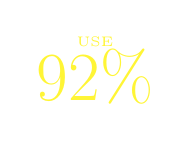
\begin{tikzpicture}
        \node [align=center, text=yellow!79] {\tiny{USE} \\ \Huge{92\%}};
    \end{tikzpicture}
\end{center}
\end{frame}

\begin{frame}
\begin{center}
    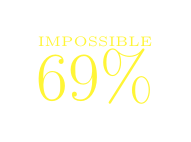
\begin{tikzpicture}
        \node [align=center, text=yellow!79] {\tiny{IMPOSSIBLE} \\ \Huge{69\%}};
    \end{tikzpicture}
\end{center}
\end{frame}

\begin{frame}
\begin{center}
    
\begin{tikzpicture}
        \node [align=center, text=yellow!79] {\tiny{DEVELOP} \\ \Huge{56\%}};
    \end{tikzpicture}
\end{center}
\end{frame}

\begin{frame}
\begin{center}
    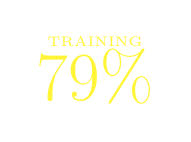
\begin{tikzpicture}
        \node [align=center, text=yellow!79] {\tiny{TRAINING} \\ \Huge{79\%}};
    \end{tikzpicture}
\end{center}
\end{frame}

\begin{frame}
\begin{center}
\movie[width=\textwidth,height=0.6\textheight,autostart, loop]{}{static/sonic.mp4}
\end{center}
\end{frame}

\begin{frame}
	\begin{center}
		\huge{\textbf{}}\\~\\
		\small{@NikoletaGlyn}\\
		\small{https://github.com/Nikoleta-v3}\\
	\end{center}
\end{frame}

\end{document}




